\documentclass[11pt, oneside]{article}   	% use "amsart" instead of "article" for AMSLaTeX format


\usepackage[letterpaper, top=10mm, left=22mm, right=22mm]{geometry}
             		% See geometry.pdf to learn the layout options. There are lots.
              		% ... or a4paper or a5paper or ... 
%\geometry{landscape}                		% Activate for rotated page geometry
%\usepackage[parfill]{parskip}    		% Activate to begin paragraphs with an empty line rather than an indent
\usepackage{graphicx}				% Use pdf, png, jpg, or eps§ with pdflatex; use eps in DVI mode
								% TeX will automatically convert eps --> pdf in pdflatex
\usepackage{amssymb,amsmath,multirow,subfigure,comment}
  
\title{\bf HPC-Homework 4}
\author{\bf \large Ya Zhu}
\date{}							% Activate to display a given date or no date
\begin{document}
\maketitle 
\begin{comment}
\section{Bug fixing}
\begin{itemize}
\item omp\_bug2: \emph{tid} and \emph{total} should be declared private for each thread.
\item omp\_bug3: \emph{\#pragma omp barrier} should not be outside the parallel directives. So comment it.
\item omp\_bug4: $a[N][N]$ may be too large to store in thread stack space and cause segment fault. So change to a smaller N.
\item omp\_bug5: if one thread has set \emph{locka} while the other has set \emph{lockb}, then when they are trying to set the other lock, deadlock happened. So unlock the lock before setting another one.
\item omp\_bug6: reduction variable should be shared by all the threads executing \emph{dotprod}. So set \emph{sum} global, and then no return variable needed for \emph{dotprod}.
\end{itemize}
\end{comment}
%\section{Experiment}
\section{Jacobi2D}
\subsection{Weak Scaling}
\begin{figure}[ht]
\centering
\subfigure[Stampede queue=\emph{development} \label{wk1}]{\includegraphics[width=0.45\linewidth]{figs/wk1.eps}}
\subfigure[Stampede queue=\emph{normal}\label{wk2}]{\includegraphics[width=0.45\linewidth]{figs/wk2.eps}}
\caption{Weak scaling with fixed $N_l = N/p$ and different number of processes.}
\end{figure}
\subsection{Strong Scaling}
\begin{figure}[ht]
\centering
\subfigure[Stampede queue=\emph{development} \label{str1}]{\includegraphics[width=0.45\linewidth]{figs/str1.eps}}
%\subfigure[Stampede queue=\emph{normal}\label{wk2}]{\includegraphics[width=0.5\linewidth]{figs/wk2.eps}}
\caption{Weak scaling with fixed $N$ and different number of processes.}
\end{figure}
\subsection{Blocking vs. Non-blocking}
\begin{table}[h]
\centering
\caption{Run time comparison for weak scaling, with $N_l=500$ and $Iter= 100000$. (Unit: second)}
\begin{tabular}{|c|c|c|c|c|}
\hline
             & 1 & 4 & 16 & 64 \\ \hline
Blocking  &  143.36 &  145.12 & 160.17 &162.43    \\ \hline
Non-Blocking &  143.95&146.34&163.18&211.26   \\ \hline
\end{tabular}
\end{table}
\begin{table}[h]
\centering
\caption{Run time comparison for strong scaling, with $N=1024$ and $Iter= 300000$. (Unit: second)}
\begin{tabular}{|c|c|c|c|c|}
\hline
             & 1 & 4 & 16 & 64 \\ \hline
Blocking     &   1803.68 & 463.60 & 117.67 & 33.46    \\ \hline
Non-Blocking &   1818.46 & 467.25 &117.84 & 32.36    \\ \hline
\end{tabular}
\end{table}
\section{Sample sort}
\begin{figure}[ht]
\centering
\subfigure[N=64 ]{\includegraphics[width=0.5\linewidth]{figs/ssort.eps}}
%\subfigure[Stampede queue=\emph{normal}\label{wk2}]{\includegraphics[width=0.5\linewidth]{figs/wk2.eps}}
\caption{Run time of sample sort paralleled on 64 cores with different number of random values per core.}
\end{figure}


\end{document}  